\chapterhead{6}{When Something Does Not Fit}{Changing the key, not forcing the fit}\label{ch6}

Every key is built from the things its maker had in front of them. Sooner or later a thing turns up that does not fit. There are two things you can do. You can force it into the nearest group. Or you can change the key.

\begin{center}
\sffamily\small\renewcommand{\arraystretch}{1.5}
\begin{tabular}{@{}p{3.4cm}p{3.7cm}p{3.7cm}@{}}
\toprule
\textbf{Model} & \textbf{What it keeps} & \textbf{What it drops}\\
\midrule
A feature & one thing about each item & every other thing\\
A yes-or-no key & a path of answers & how items differ in other ways\\
A group & what the members share & how they differ\\
A nested circle & groups inside groups & the details of each item\\
\bottomrule
\end{tabular}
\end{center}

\subhead{The bat that broke a key}
Suppose a key says: ``Does it have wings? Yes, it is a bird. No, it is a mammal.'' A bat has wings, so the key calls it a bird. But a bat has fur and feeds its young milk. The key was built for the birds and the cats it knew.

\begin{center}
\begin{tikzpicture}
  \node[bigcir,minimum size=2.3cm] (a) at (0,0) {}; \node[font=\sffamily\scriptsize,align=center] at (0,0) {old key:\\``wings?''};
  \node[wrapcir,minimum size=2.9cm] (w) at (5.4,0) {}; \node[font=\sffamily\scriptsize,align=center] at (5.4,0) {new key:\\``feathers?''};
  \draw[popA] (a) -- node[above,note] {bat breaks it} (w);
  \node[note,anchor=west,text width=3cm,align=left] at (7.2,0) {\textbf{kept:} the old key, wrapped\\\textbf{set aside:} the wrong question};
\end{tikzpicture}
\end{center}

\begin{tryit}{Break your own key}
Take the key you wrote in Chapter~4 or~5. Find or imagine one thing that does not fit it. What happens? Write the new question that fixes it.\par\medskip
The thing that broke it: \wline[6cm]\\[8pt]
Which question failed? \wline[6cm]\\[8pt]
The new question: \wline[6cm]
\end{tryit}

\begin{worked}{The worm in the animal key}
In Chapter~5, a worm has no legs, no feathers or fur, no shell and no fins. Q1 no, Q3 no, Q4 no, Q6 no, Q7 no. It ends at frog. But a worm is not a frog.\\
The fix: add a new question before Q7, ``Does it have legs?'' A worm answers no and goes to a new group. The old key is wrapped by the new one.
\end{worked}

\begin{multix}[hmm]\multixbot[hmm]\tcblower
The worm ended in the frog group. The key must be right, so the worm must be a frog. I trust the key. Do you?
\end{multix}

\trust{We tried a new specimen on the old key, saw where it ended and fixed the key when the result looked wrong.}
{The worm and the bat each exposed a missing question, and the fixes kept every earlier animal where it was.}
{That the new key is finished. Some other animal will break it too. A key is always a model for the things it has met.}

\begin{keepbox}
We changed a key when something did not fit. \textbf{We kept} \wline[3.4cm] \textbf{and we set aside} \wline[3.4cm].
\end{keepbox}

\clearpage

\begin{puzzle}{The bat}
A key says ``wings? yes: bird, no: mammal''. Where does it put a bat? \wline[3cm] Why is that wrong? \wline[5cm]
\end{puzzle}

\begin{puzzle}{The worm}
Which new question separates the worm from the frog? \wline[6cm]
\end{puzzle}

\begin{puzzle}{Change or force?}
Is it better to force a surprise thing into the nearest group or to change the key? \wline[3cm] Why? \wline[4cm]
\end{puzzle}

\begin{puzzle}{A new bug}
A new bug has wings, spots and antennae that are neither long nor short. Does the bug key sort it? \wline[2cm] What would you change? \wline[4cm]
\end{puzzle}

\begin{puzzle}{Wrap the key}
Draw the new question wrapped around the old key.
\begin{center}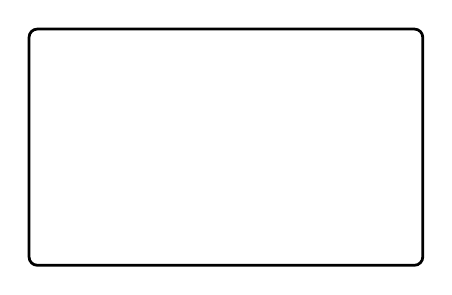
\begin{tikzpicture}\draw[line width=1pt,rounded corners=3pt] (0,0) rectangle (5,3); \end{tikzpicture}\end{center}
\end{puzzle}

\clearpage

\begin{puzzle}{Eight groups}
A key uses wings, spots and antennae. How many different groups can it make? \wline[1.6cm]
\end{puzzle}

\begin{puzzle}{Already there}
A new bug J has no wings, no spots and long antennae. Which bug in the tray matches J exactly? \wline[1.6cm]
\end{puzzle}

\begin{puzzle}{Sentence check}
Mark S if the evidence supports it, G if it is a guess, and B if it is too big.\\
(a) ``The key put the bat with the birds.'' \wline[1cm]\\
(b) ``Wings are a poor feature for sorting animals.'' \wline[1cm]\\
(c) ``No key works for every animal ever.'' \wline[1cm]
\end{puzzle}

\begin{puzzle}{Flying}
Birds and bats both fly. What feature would separate them? \wline[6cm]
\end{puzzle}

\clearpage

\begin{puzzle}{Thirty-two things}
You need to separate 32 things, one to a group. How many questions in a row? \wline[1.6cm]
\end{puzzle}

\begin{puzzle}{Model or real?}
Write M for model and R for real thing.\\
(a) the key \wline[1cm] \quad (b) the bat \wline[1cm] \quad (c) the tray picture \wline[1cm]
\end{puzzle}

\begin{puzzle}{Agreement}
Two people used a key on ten things and landed in the same group on all ten. Does that prove the key is perfect? \wline[2cm] Why not? \wline[4cm]
\end{puzzle}

\begin{puzzle}{Trust}
A student says her key is perfect because she used it herself. What would you ask her to do? \wline[6cm]
\end{puzzle}

\clearpage

\begin{puzzle}{Draw a key for four}
Draw a two-question key for four things you choose. Label the questions.
\begin{center}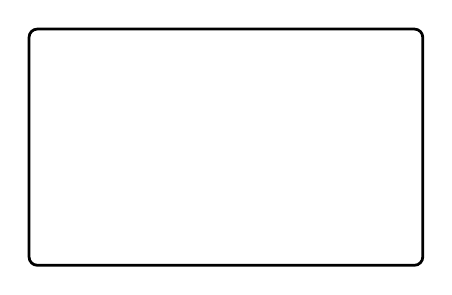
\begin{tikzpicture}\draw[line width=1pt,rounded corners=3pt] (0,0) rectangle (5,3); \end{tikzpicture}\end{center}
\end{puzzle}

\begin{puzzle}{Draw the split}
Draw a circle of 16 splitting into two of 8, and one of the 8s splitting again.
\begin{center}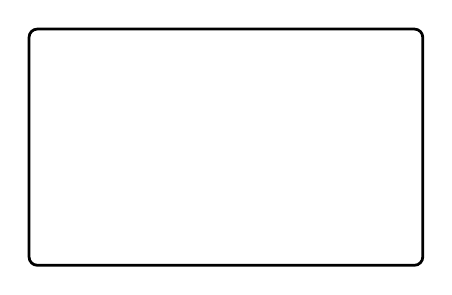
\begin{tikzpicture}\draw[line width=1pt,rounded corners=3pt] (0,0) rectangle (5,3); \end{tikzpicture}\end{center}
\end{puzzle}

\begin{puzzle}{Draw the wrap}
Draw a circle around ``wings? bird'' and write the fixed question outside.
\begin{center}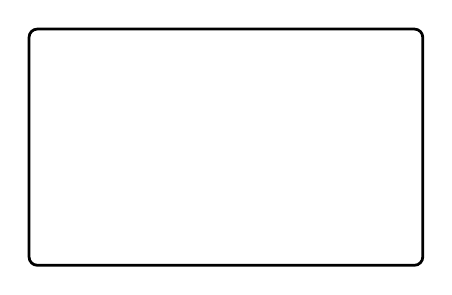
\begin{tikzpicture}\draw[line width=1pt,rounded corners=3pt] (0,0) rectangle (5,3); \end{tikzpicture}\end{center}
\end{puzzle}

\clearpage
\thispagestyle{fancy}\label{slop}
\subhead{Slop check}
Slop is hasty, gaudy work that forgot to take care. It can be made by a person or a machine, quickly or slowly. What matters is whether the work shows care for three things:
\begin{itemize}[leftmargin=1.6em]
\item \textbf{Salient:} Is the main point easy to see?
\item \textbf{Simple:} Is there anything that does nothing but get in the way?
\item \textbf{Relevant:} Does everything on the page help answer the question?
\end{itemize}

Here is a hasty poster about sorting. Study it, then decide what is wrong.

\begin{center}
\begin{tikzpicture}[scale=0.97]
  \fill[yellow!40,draw=purple!80!black,line width=3pt] (0,0) rectangle (11.4,7.6);
  \node[star,star points=12,fill=red!60,draw=blue,line width=2pt,minimum size=2.2cm,font=\bfseries\scriptsize,rotate=10,text=yellow] at (1.4,6.2) {WOW!!!};
  \node[font=\itshape\bfseries\Large,text=teal,rotate=-4] at (6.4,6.8) {SoRtInG Is MaGiC};
  \node[font=\ttfamily\tiny,text=orange] at (6.4,6.15) {(things maybe? who knows)};
  \foreach \x/\h/\c in {3/1.2/red,5.3/3.2/blue,7.6/5.0/green}{
    \fill[\c,draw=black] (\x,0.9) rectangle (\x+1.3,0.9+\h);
  }
  \node[font=\tiny,text=black,rotate=60] at (9.8,3) {number number number};
  \foreach \x/\y in {1.2/1.5,1.6/4.2,10.2/5.6,0.8/3}{\node[star,star points=5,fill=yellow,draw=red,minimum size=0.6cm] at (\x,\y) {};}
  \node[font=\tiny,text=lime!50!black] at (5.4,0.45) {sort it!!!  best sorting ever!!!  wow  wow};
\end{tikzpicture}
\end{center}

\begin{slopbox}
\textbf{(a)} What is the poster's main point? Can you tell?\\[3pt]\rule{\linewidth}{0.5pt}\\[6pt]
\textbf{(b)} Name two things that are not simple, because they only distract.\\[3pt]\rule{\linewidth}{0.5pt}\\[6pt]
\textbf{(c)} Name two things that are missing, so the bars cannot be read.\\[3pt]\rule{\linewidth}{0.5pt}\\[6pt]
\textbf{(d)} Which part is not relevant to sorting at all?\\[3pt]\rule{\linewidth}{0.5pt}
\end{slopbox}

\clearpage
\thispagestyle{fancy}
\subhead{Now you try}
On a separate sheet, redraw a clear bar chart of how the twelve buttons were sorted by colour: red 3, blue 4 and white 5. Give it a title, label the axes with units, use one or two calm colours, and delete everything that does not help. Check it against the three words: salient, simple, relevant.

\begin{center}
\begin{tikzpicture}
  \draw[ink!70,line width=1pt,rounded corners=3pt] (0,0) rectangle (11.4,1.0);
  \node[font=\sffamily\small,anchor=west] at (0.2,0.5) {Title:};
  \draw[line width=1.3pt] (1,1.6) -- (1,9.6);\draw[line width=1.3pt] (1,1.6) -- (11,1.6);
  \foreach \y in {2.6,3.6,...,8.6}{\draw[gray!40] (1,\y) -- (11,\y);}
  \node[font=\sffamily\scriptsize,rotate=90] at (0.3,5.6) {label and unit here};
  \node[font=\sffamily\scriptsize] at (6,1.3) {label what the axis stands for};
\end{tikzpicture}
\end{center}

\clearpage
\thispagestyle{fancy}
\subhead{What did we keep, across the whole book?}
For each chapter, say one thing that was simplified, what was kept, and what was set aside. A sample is done for you.

\renewcommand{\arraystretch}{2.3}
\begin{center}\sffamily\scriptsize
\begin{tabularx}{\textwidth}{|>{\bfseries}p{2.1cm}|X|X|X|}
\hline
\textbf{Chapter} & \textbf{What we simplified} & \textbf{What we kept} & \textbf{What we set aside} \\ \hline
1 Many ways to sort & a pile as groups & the feature we chose & every other feature \\ \hline
2 Features that matter & a bug as a few features & clear splitters & fuzzy features \\ \hline
3 A yes-or-no key & a sort as questions & the path of answers & other differences \\ \hline
4 Trading keys & a key as shared rules & agreement between people & fuzzy lines \\ \hline
5 Groups inside groups & animals as nested circles & the groups that nest & details of each animal \\ \hline
6 When something does not fit & & & \\ \hline
\end{tabularx}
\end{center}

\begin{multix}[wow]\multixbot[wow]\tcblower
Everything you sorted in this book was a simplification of something. A key is allowed to drop things, as long as you say which. Next time something does not fit, you will change the key.
\end{multix}

\clearpage
\thispagestyle{fancy}
\subhead{Write a sorting report}
\begin{tcolorbox}[enhanced,colback=white,colframe=ink!60,boxrule=1pt,arc=2mm,left=8pt,right=8pt,top=5pt,bottom=5pt]
\sffamily\small
\begin{enumerate}[leftmargin=1.6em,itemsep=0.2em]
\item \textbf{What I looked at.}
\item \textbf{What I changed, measured and kept the same.}
\item \textbf{My readings.} All of them.
\item \textbf{My answer.} With how many agreed.
\item \textbf{What I kept and what it hides.}
\end{enumerate}
\end{tcolorbox}
\vspace{4pt}
Pick one key from this book and write a report on it. Use the lines below.\par\medskip
\foreach \i in {1,...,12}{\rule{\linewidth}{0.4pt}\\[18pt]}
\clearpage

\thispagestyle{fancy}
\subhead{Tests to try}
Pick one and design it with the habits from this book: change one thing, keep the rest the same, repeat, and check with a friend.
\begin{enumerate}[leftmargin=1.6em,itemsep=0.5em]
\item Does a key with fewer questions agree as often as one with more?
\item Do two friends sort the same ten leaves the same way?
\item Which feature best splits a pile of shells: colour, shape or size?
\item Can a younger child use your key and agree with you?
\item How many questions does a key need for 20 things?
\item Does the order of the questions change how many things end up in each group?
\end{enumerate}
\medskip
Write the test you pick:\par\medskip
\foreach \i in {1,...,6}{\rule{\linewidth}{0.4pt}\\[16pt]}
Change: \wline[3cm] Measure: \wline[3cm] Keep the same: \wline[3cm]
\clearpage

\thispagestyle{fancy}
\subhead{A week of sorting}
Each day, notice one group of things and the feature that makes it a group.\par\medskip
\renewcommand{\arraystretch}{3.2}
\begin{tabularx}{\linewidth}{|>{\sffamily\small\bfseries}p{1.8cm}|X|X|}
\hline
Day & The group & The feature \\ \hline
Mon & & \\ \hline
Tue & & \\ \hline
Wed & & \\ \hline
Thu & & \\ \hline
Fri & & \\ \hline
Sat & & \\ \hline
Sun & & \\ \hline
\end{tabularx}
\clearpage

\thispagestyle{fancy}
\subhead{Questions I still have}
Write what you still wonder about sorting. Then pick one and think how to test it.\par\medskip
\foreach \i in {1,...,16}{\rule{\linewidth}{0.4pt}\\[16pt]}
\clearpage
